\documentclass[a4paper,12pt,titlepage,oneside]{article}

\usepackage[italian]{babel}
\usepackage[utf8]{inputenc}
\usepackage{listings} 
\usepackage{cite}
\lstset{
    literate={~} {$\sim$}{1}
}
\usepackage{amsmath,amssymb,amsfonts,amsthm,graphicx,mathrsfs,braket}
\usepackage{hyperref}
\usepackage{times}
\usepackage[left=2.5cm, right=2.5cm]{geometry}
\usepackage{parskip}
\usepackage{xcolor}
\hypersetup{colorlinks=false,
allbordercolors=white}
\setcounter{secnumdepth}{4} 
\setcounter{tocdepth}{3}
\linespread{1.5}
\begin{document}
\newcommand\tab[1][1cm]{\hspace*{#1}}
\thispagestyle{empty}
\begin{figure}
	\centering
	\vspace*{-2cm}	
	
\includegraphics[scale=0.4]{logo.png}
	\label{fig:logo}
\end{figure}
\centerline{{\LARGE UNIVERSIT\`{A} DEGLI STUDI DI CATANIA}}
\centerline{DIPARTIMENTO DI MATEMATICA E INFORMATICA} \centerline{CORSO DI LAUREA MAGISTRALE IN INFORMATICA}
\centerline{\rule{16cm}{0.2mm}}\vspace*{2cm}
\centerline{\huge{UNCAPACITATED FACILITY LOCATION PROBLEM}}
\centerline{\huge{}}
\centerline{\huge{WITH}}
\centerline{\huge{}}
\centerline{\huge{IMMUNOLOGICAL ALGORITHM}}
\vspace*{2cm}
\centerline{\rule{5cm}{0.2mm}}\medskip
\centerline{\Large{PROGETTO DI COMPUTAZIONE NATURALE}}
\centerline{\rule{5cm}{0.2mm}}
\vspace*{4cm}

\centerline{\Large{Andrea Sequenzia}}
\centerline{\Large{Matricola: W82000160}}


\vspace*{2cm}

%\vspace{1cm}
\enlargethispage{10cm}
\centerline{\rule{16cm}{0.2mm}} 
\centerline{ANNO ACCADEMICO 2018/2019} 
\newpage
\tableofcontents
\newpage

\section{Introduzione}


\section{Definizione del problema}
In un problema UFLP, ci sono $m$ clienti da servire ed $n$ possibili location dove poter stabilire delle facilities che servano i clienti e soddisfare la domanda. Ogni facility $i$ ha un costo fisso di installazione $f_{i}$. Un costo di trasporto $c_{ij}$ per servire il il cliente $j$ dalla facility $i$. Le facility non hanno limiti nelle capacità di quanto possono servire e non ci devono essere clienti non soddisfatti. L'obiettivo finale è quello di stabilire quali facility attivare, soddisfando tutti i clienti, minimizzando il costo per ottenere ciò. Formalmente:

\begin{equation*}
\begin{aligned}
& \underset{}{\text{minimize}}
& & \sum_{i=1}^{n} \sum_{j=1}^{m}c_{ij}x_{ij} + \sum_{i=1}^{n}f_{i}y_{i} \\
& \text{subject to}
& & \sum_{i=1}^{n}x_{ij}=1, \quad j=1,...,m, \\
& & & x_{ij}\leq y_{i}, \quad i=1,...,n, j=1,...,m,\\
& & &  x_{ij},y_i=0,1,\quad i=1,...,n, j=1,...,m
\end{aligned}
\end{equation*}
dove \\
$c_{ij} =$ il costo per soddisfare la domanda del cliente $j$ dalla facility $i$; \\
$f_{i} =$ il costo per stabilire la facility nella location $i$ \\

$x_{ij}=\left\{\begin{aligned}
 & 1 \quad \text{se il cliente j viene servito dalla facility i},\\ 
 & 0 \quad altrimenti;
\end{aligned}\right.$

$y_{i}=\left\{\begin{aligned}
 & 1 \quad \text{se la facility è stabilita nella location i},\\ 
 & 0 \quad altrimenti;
\end{aligned}\right.$

\begin{figure}
  \centering
  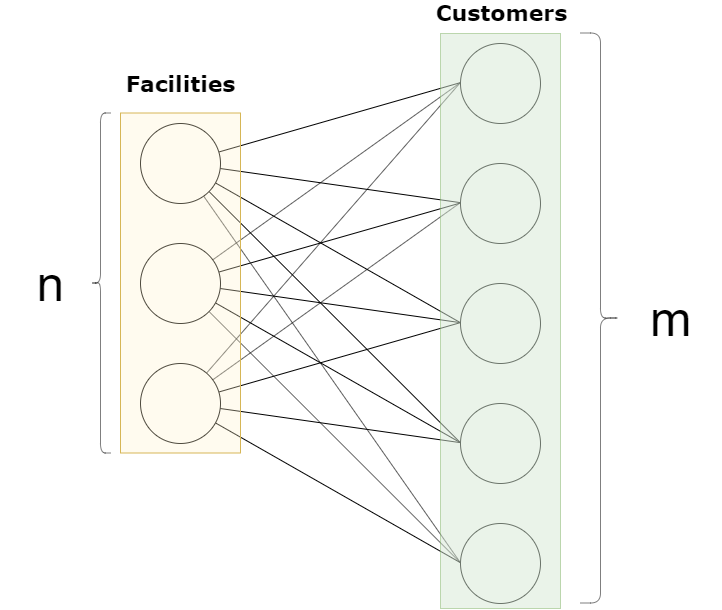
\includegraphics[scale=.3]{UFLP_Sample.png}
  \caption{Esempio problema UFLP}
\end{figure}

Il problema può essere matematicamente decomposto in due sottoproblemi indipendenti \cite{Sultan1999}:
\begin{enumerate}
\item \textbf{Location}, ovvero le facilities da stabile ($y_{i}$)
\item \textbf{Allocation}, per le facility stabilite, determinare la distribuzione e quindi quali archi usare per ogni customer ($x_{ij}$) 
\end{enumerate}

Per ogni soluzione del problema di Location, una soluzione ottima può essere ottenuta per il problema Allocation. Dato un vettore $y$, può essere ottenuto un assegnamento ottimale delle $x_{ij}$ usando la seguente formula:

\begin{equation*}
\begin{aligned}
& k:\min_{k}c_{kj}, \quad k = 1,...,n \\
& x_{ij}=\left\{\begin{aligned}
& 1 \quad \text{se i=k},\\ 
& 0 \quad altrimenti;
\end{aligned}\right.
\end{aligned}
\end{equation*}

Quindi il problema si riduce a determinare l'assegnamento di facilities ottimale.
\section{Algoritmo immunologico}
Un algoritmo immunologico è un algoritmo basato sul clonal selection principle, esso è un ottimo esempio di strategia intelligente in cui l'adattamento opera a livello locale, mentre un comportamento complesso agisce a livello globale. L'idea di questa tipologia di algoritmo deriva dal sistema immunitario naturale, in particolare da come le cellule si adattano per legarsi ed eliminare
entità straniere, meglio conosciute come Antigene. Questo algoritmo è basato su due entità: gli \textbf{antigeni} che rappresentano il problema da affrontare e le \textbf{B cell} (Linfocita B) che rappresentano un punto nello spazio di ricerca \cite{Pavone}. L'algoritmo crea una popolazione di B cell, esse cresceranno e si perfezioneranno nel corso di un numero prefissato di generazioni, morendo quando hanno raggiunto un'età prefissata. La qualità delle B cell si valuta attraverso una funzione di fitness. Gli operatori usati da questo algoritmo sono in sequenza i seguenti:
\begin{enumerate}
\item \textbf{Cloning}: questo operatore simula il meccanismo di proliferazione di un sistema immunitario. Esso genera una popolazione intermedia $P^{(clo)}$ copiando \textit{dup} volte ogni B cell, assegnando un'età, la nuova popolazione così fatta sarà delle dimensioni \textit{$d \times dup$}. 
\item \textbf{Inversely Hypermutation}: il compito di questo operatore è quello di esplorare il vicinato di ogni clone creato dal precedente operatore. Ciò viene compiuto eseguendo $M$ mutazioni ad ogni elemento di $P^{(clo)}$. Per determinare $M$, viene adottata una legge inversamente proporzionale al valore della fitness: più piccolo (minimizzazione) è il valore valore della funzione di fitness, meno mutazioni saranno fatte alla B cell. Dato un clone $x$, per determinare il valore $M$ è necessaria la seguente formula:
\begin{equation}
\alpha=e^{-\rho\hat{f}(x)}
\end{equation}
dove $\alpha$ rappresenta il mutation rate,$\rho$ lo shape del mutation rate e $\hat{f}(x)$ è il valore della funzione di fitness normalizzato tra $[0,1]$. Il numero di mutazioni $M$ è dato da:
\begin{equation}
M = \lfloor(\alpha \times l) + 1 \rfloor
\end{equation}
dove $l$ è la lunghezza di una B cell. 
\item \textbf{Aging}: questo operatore aiuta l'algoritmo a saltare via dagli ottimi locali. Per ottenere ciò, rimuove le vecchie B cell dalla popolazione iniziale e da quella ipermutata. L'eliminazione avviene quando l'età (che viene incrementata ad ogni fine generazione) raggiunge l'età massima ($\tau_{b}$). Così facendo, si produce alta diversità e si aiuta l'algoritmo ad evitare le convergenze premature. Viene anche fatta un eccezione nella rimozione, ovvero lasciare la migliore soluzione nella popolazione anche se ha raggiunto la massima età. Questa variante viene chiamata \textit{elitist aging operator}.
\item \textbf{($\mathbf{\mu + \lambda}$)-Selection}:
\end{enumerate}
\section{Implementazione}

\section{Esperimenti}
\section{Conclusioni}
\newpage
\bibliography{bibliografia}{}
\bibliographystyle{plain}
\end{document}
